\documentclass[aspectratio=169,11pt]{beamer}

\usetheme{metropolis}
\metroset{progressbar=frametitle, sectionpage=progressbar, numbering=none}

\usepackage[ngerman]{babel}
\usepackage{tikz}
\usetikzlibrary{arrows.meta,positioning,calc,decorations.pathreplacing,fit,backgrounds}
\usepackage{fontawesome5}

% BFH / Metropolis preamble for the WDDA regression walkthrough deck.
% Brand colours and logo handling adapted from the BSAN "litmus/bfh" theme.

% === BRAND COLORS ===
\usepackage{xcolor}
\definecolor{LitmusPrimary}{HTML}{697D91}
\definecolor{LitmusSecondary}{HTML}{FAC300}
\definecolor{LitmusAccent}{HTML}{699673}
\definecolor{LitmusDark}{HTML}{697D91}
\definecolor{LitmusCorrect}{HTML}{699673}
\definecolor{LitmusIncorrect}{HTML}{B41428}
\definecolor{LitmusAlert}{HTML}{F7931E}

% === GRAPHICS / LOGOS ===
\usepackage{graphicx}
\newcommand{\litmuslogo}{bfh-logo.pdf}
\newcommand{\litmoslockup}{bfh-lockup.pdf}

% === MATH ===
\usepackage{amsmath,amssymb}
\usepackage{booktabs}

% === CODE LISTINGS (R) ===
\usepackage{listings}
\lstdefinestyle{Rcode}{
  language=R,
  basicstyle=\ttfamily\footnotesize,
  keywordstyle=\color{LitmusAccent}\bfseries,
  commentstyle=\color{gray}\itshape,
  stringstyle=\color{LitmusPrimary},
  numberstyle=\tiny\color{gray},
  frame=single,
  framerule=0.5pt,
  rulecolor=\color{LitmusAccent!30},
  backgroundcolor=\color{LitmusDark!5},
  breaklines=true,
  showstringspaces=false,
  columns=fullflexible,
  keepspaces=true,
}
% Console-output style (no syntax colours)
\lstdefinestyle{Rout}{
  basicstyle=\ttfamily\footnotesize\color{black!80},
  frame=single,
  framerule=0.5pt,
  rulecolor=\color{LitmusPrimary!25},
  backgroundcolor=\color{LitmusPrimary!4},
  breaklines=true,
  showstringspaces=false,
}
\lstnewenvironment{rcode}{\lstset{style=Rcode}}{}
\lstnewenvironment{rout}{\lstset{style=Rout}}{}

% === METROPOLIS / BEAMER TWEAKS ===
\setbeamercolor{progress bar}{fg=LitmusSecondary}
\setbeamercolor{alerted text}{fg=LitmusAlert}
\setbeamercolor{example text}{fg=LitmusAccent}
\setbeamercolor{frametitle}{bg=LitmusPrimary}

% Footer logo on regular slides (skip the title page)
\setbeamertemplate{frame footer}{%
  \ifnum\value{page}>1\relax
    \IfFileExists{\litmuslogo}{\includegraphics[height=0.3cm]{\litmuslogo}}{}%
  \fi
}

% Title page with the BFH lockup logo
\makeatletter
\setbeamertemplate{title page}{
  \begin{minipage}[b][\paperheight]{\textwidth}
    \vfill
    \ifx\inserttitle\@empty\else\usebeamertemplate*{title}\fi
    \ifx\insertsubtitle\@empty\else\usebeamertemplate*{subtitle}\fi
    \usebeamertemplate*{title separator}
    \ifx\beamer@shortauthor\@empty\else\usebeamertemplate*{author}\fi
    \ifx\insertdate\@empty\else\usebeamertemplate*{date}\fi
    \ifx\insertinstitute\@empty\else\usebeamertemplate*{institute}\fi
    \vfill
    \IfFileExists{\litmoslockup}{\includegraphics[height=1cm]{\litmoslockup}}{}
    \vspace*{1em}
  \end{minipage}
}
\makeatother

% === CONTENT BOXES (concept / takeaway / warning) ===
\usepackage{tcolorbox}
\tcbuselibrary{skins}
\newtcolorbox{konzept}[1][Kernkonzept]{
  colback=LitmusAccent!6, colframe=LitmusAccent,
  fonttitle=\bfseries, title={#1}, boxrule=0.8pt, arc=2pt,
  left=4pt, right=4pt, top=3pt, bottom=3pt,
}
\newtcolorbox{merke}[1][Merke]{
  colback=LitmusSecondary!12, colframe=LitmusSecondary!85!black,
  fonttitle=\bfseries, title={#1}, boxrule=0.8pt, arc=2pt,
  left=4pt, right=4pt, top=3pt, bottom=3pt,
}
\newtcolorbox{warnung}[1][Achtung]{
  colback=LitmusIncorrect!6, colframe=LitmusIncorrect,
  fonttitle=\bfseries, title={#1}, boxrule=0.8pt, arc=2pt,
  left=4pt, right=4pt, top=3pt, bottom=3pt,
}


\title{Regression Schritt für Schritt}
\subtitle{Drei Übungen aus den Serien 5, 6 und 7 --- WDDA FS 2026}
\author{Ulrich Matter}
\date{}
\institute{Berner Fachhochschule --- Datenmanagement und Datenanalyse}

\begin{document}

\frame{\titlepage}

% ============================================================
\begin{frame}{Worum geht es heute?}
Wir lösen \alert{drei ausgewählte Übungen} --- und lernen dabei die
Kernideen der Regression kennen:

\vspace{0.4cm}
\begin{columns}[T]
\begin{column}{0.32\textwidth}
  \begin{konzept}[Serie 5]
  \textbf{Einfache Regression}\\[2pt]
  Diamantringe: eine Gerade durch die Daten --- und ein
  \emph{Schnäppchen-Test}.
  \end{konzept}
\end{column}
\begin{column}{0.32\textwidth}
  \begin{konzept}[Serie 6]
  \textbf{Multiple Regression}\\[2pt]
  Download: Was passiert, wenn zwei Prädiktoren fast
  \emph{dasselbe} messen?
  \end{konzept}
\end{column}
\begin{column}{0.32\textwidth}
  \begin{konzept}[Serie 7]
  \textbf{Inferenz}\\[2pt]
  Advertising: Wie \emph{sicher} sind unsere Schätzungen und
  Prognosen?
  \end{konzept}
\end{column}
\end{columns}

\vspace{0.4cm}
Roter Faden: \textbf{Gerade anpassen $\rightarrow$ mehrere Prädiktoren
$\rightarrow$ Unsicherheit ehrlich beziffern.}
\end{frame}

\begin{frame}{Lernziele}
Nach diesen drei Übungen können Sie:
\begin{enumerate}
  \item eine \alert{einfache lineare Regression} in R aufstellen und
        Achsenabschnitt, Steigung sowie $R^2$/RSE interpretieren;
  \item ein \alert{Prognoseintervall} nutzen, um eine konkrete
        Entscheidung zu treffen;
  \item \alert{marginale} und \alert{partielle} Steigungen unterscheiden
        und \alert{Multikollinearität} erkennen;
  \item \alert{Konfidenzintervalle} klassisch und per \alert{Bootstrap}
        berechnen und vergleichen;
  \item mit \alert{t-Test} und \alert{F-Test} entscheiden, welche
        Prädiktoren ins Modell gehören;
  \item \alert{Konfidenz-} und \alert{Prognoseintervall} auseinanderhalten.
\end{enumerate}
\end{frame}

% ============================================================
\section{Serie 5 --- Einfache lineare Regression}
% ============================================================

\begin{frame}{Die Aufgabe: Diamantringe}
\textbf{Datensatz \texttt{Diamonds Rings}} (48 Ringe): Gewicht in Karat,
Listenpreis in Singapur-Dollar (SGD).

\vspace{0.3cm}
Wir wollen:
\begin{enumerate}
  \item den Zusammenhang \textbf{Preis $\sim$ Gewicht} modellieren,
  \item Achsenabschnitt, Steigung und Modellgüte interpretieren,
  \item den Preisunterschied zwischen 0.25 und 0.35\,ct schätzen,
  \item entscheiden: Ist ein Ring mit \textbf{0.18\,ct für 325 SGD} ein
        \alert{Schnäppchen}?
\end{enumerate}

\vspace{0.3cm}
\begin{merke}[Leitfrage]
Wie zieht man die \emph{beste} Gerade durch eine Punktwolke --- und was
heisst „beste``?
\end{merke}
\end{frame}

\begin{frame}{Kernkonzept: Was ist eine lineare Regression?}
Wir beschreiben den Preis als \alert{Gerade} im Gewicht:
\[
  \hat{y} \;=\; \underbrace{b_0}_{\text{Achsenabschnitt}}
  \;+\; \underbrace{b_1}_{\text{Steigung}} \cdot x
\]

\begin{columns}[T]
\begin{column}{0.5\textwidth}
\begin{itemize}
  \item $x$ = Gewicht (Karat), $\hat y$ = geschätzter Preis
  \item $b_0$: Modellpreis bei $x = 0$
  \item $b_1$: \textbf{Mehrpreis pro zusätzlichem Karat}
\end{itemize}
\end{column}
\begin{column}{0.5\textwidth}
\begin{itemize}
  \item Die Abweichung jedes Punkts von der Geraden heisst
        \alert{Residuum} $e_i = y_i - \hat y_i$
  \item R berechnet $b_0, b_1$ mit einer Zeile: \texttt{lm()}
\end{itemize}
\end{column}
\end{columns}

\vspace{0.3cm}
\begin{merke}
Korrelation sagt „\emph{es gibt} einen Zusammenhang``. Regression sagt
\textbf{wie stark} und erlaubt \textbf{Prognosen}.
\end{merke}
\end{frame}

\begin{frame}[fragile]{Schritt 1--2: Daten einlesen und ansehen}
\begin{columns}[T]
\begin{column}{0.52\textwidth}
\begin{rcode}
library(readxl)
diamonds <- read_excel(
  "WDDA_05.xlsx",
  sheet = "Diamonds Rings")
names(diamonds) <- c("weight", "price")

plot(diamonds$weight, diamonds$price)
\end{rcode}
\vspace{0.2cm}
\small Immer zuerst \textbf{plotten}: Ist der Zusammenhang überhaupt
ungefähr linear? Hier: ja, klar steigend.
\end{column}
\begin{column}{0.46\textwidth}
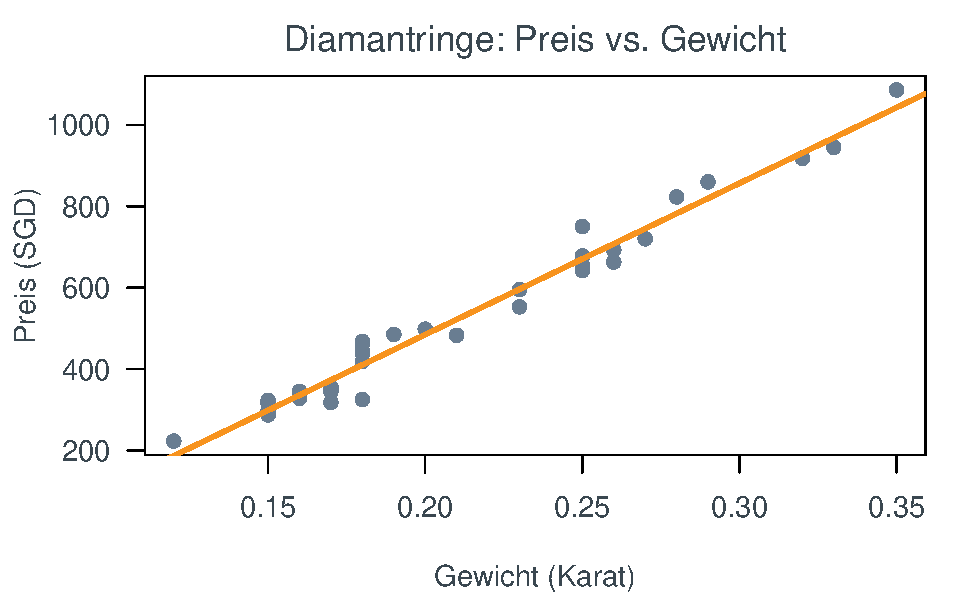
\includegraphics[width=\linewidth]{figures/dr_scatter.pdf}
\end{column}
\end{columns}
\end{frame}

\begin{frame}{Kernkonzept: Die Methode der kleinsten Quadrate}
\begin{columns}[T]
\begin{column}{0.46\textwidth}
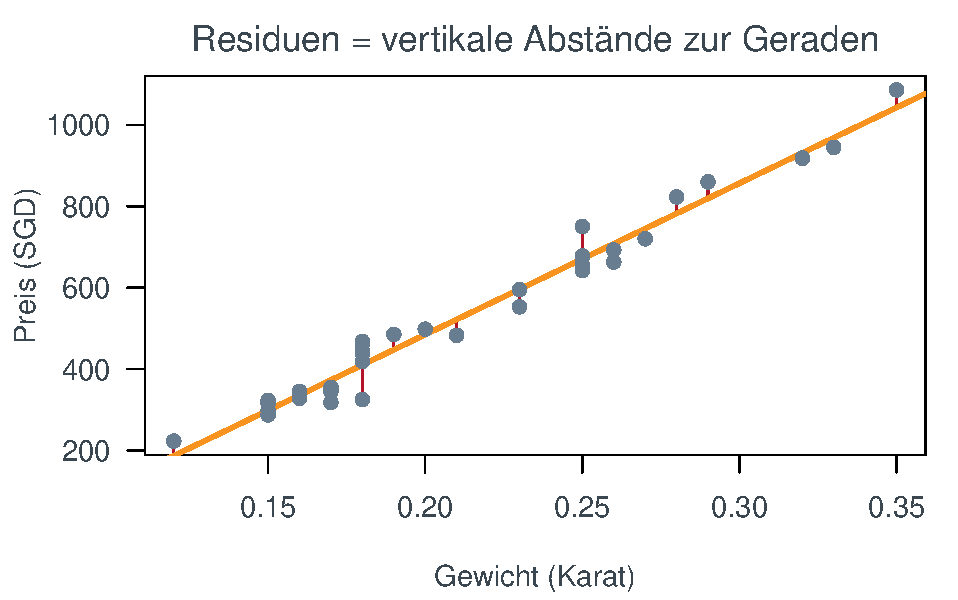
\includegraphics[width=\linewidth]{figures/dr_leastsquares.pdf}
\end{column}
\begin{column}{0.5\textwidth}
R wählt $b_0, b_1$ so, dass die \alert{Summe der quadrierten Residuen}
minimal wird:
\[
  \min_{b_0,\,b_1}\ \sum_{i=1}^{n}\bigl(y_i - \hat y_i\bigr)^2
  \;=\; \min \sum_i e_i^2
\]
\begin{itemize}
  \item rote Linien = Residuen $e_i$
  \item Quadrieren $\Rightarrow$ grosse Abweichungen zählen stärker
  \item Ergebnis: \textbf{eine eindeutige} beste Gerade
\end{itemize}
\end{column}
\end{columns}
\end{frame}

\begin{frame}[fragile]{Schritt 3: Modell schätzen mit \texttt{lm()}}
\begin{rcode}
mod_dr <- lm(price ~ weight, data = diamonds)
summary(mod_dr)
\end{rcode}
\begin{rout}
Coefficients:
            Estimate Std. Error t value Pr(>|t|)
(Intercept)  -259.63      17.32  -14.99   <2e-16 ***
weight       3721.02      81.79   45.50   <2e-16 ***
---
Residual standard error: 31.84 on 46 degrees of freedom
Multiple R-squared:  0.9783
\end{rout}
\vspace{0.15cm}
\centering
$\hat{\text{price}} = -259{,}63 + 3721{,}02 \cdot \text{weight}$
\end{frame}

\begin{frame}{Schritt 3: Was bedeuten die Koeffizienten?}
\[
  \hat{\text{price}} = \underbrace{-259{,}63}_{b_0}
  + \underbrace{3721{,}02}_{b_1} \cdot \text{weight}
\]
\begin{columns}[T]
\begin{column}{0.5\textwidth}
\textbf{Steigung $b_1 = 3721$ SGD/ct}
\begin{itemize}
  \item Jedes zusätzliche Karat $\to$ rund \textbf{3721 SGD} mehr
  \item das ist die zentrale, sinnvolle Zahl
\end{itemize}
\end{column}
\begin{column}{0.5\textwidth}
\textbf{Achsenabschnitt $b_0 = -259$ SGD}
\begin{itemize}
  \item rechnerischer Preis bei 0\,ct --- ein \alert{negativer} Preis
  \item \textbf{nicht sinnvoll interpretierbar}: 0\,ct liegt weit
        ausserhalb der Daten (0.12--0.35\,ct)
\end{itemize}
\end{column}
\end{columns}
\vspace{0.3cm}
\centering
$b_1$ ist die zentrale Zahl --- mit $b_0$ ist Vorsicht geboten
(nächste Folie).
\end{frame}

\begin{frame}{Schritt 3: Vorsicht beim Achsenabschnitt}
$b_0 = -259$ SGD ist der Modellwert bei \textbf{0 Karat} --- ein
\alert{negativer Preis}. Kein Widerspruch:

\vspace{0.2cm}
\begin{columns}[T]
\begin{column}{0.5\textwidth}
\textbf{Warum?}
\begin{itemize}
  \item Daten nur von \textbf{0.12--0.35\,ct}
  \item $x = 0$ liegt weit ausserhalb $\Rightarrow$ \textbf{Extrapolation}
\end{itemize}
\end{column}
\begin{column}{0.5\textwidth}
\textbf{Was zählt?}
\begin{itemize}
  \item die \alert{Steigung} $b_1$
  \item Prognosen \emph{innerhalb} der Daten
\end{itemize}
\end{column}
\end{columns}
\vspace{0.2cm}
\begin{warnung}
$b_0$ nie blind interpretieren --- $x=0$ ist reine Extrapolation.
\end{warnung}
\end{frame}

\begin{frame}{Kernkonzept: Wie gut ist das Modell? ($R^2$, RSE)}
\textbf{Idee:} Zerlege die gesamte Streuung der Preise (TSS) in einen
\emph{erklärten} und einen \emph{unerklärten} Teil (RSS).
\[
  R^2 = 1 - \frac{\text{RSS}}{\text{TSS}}
      = 1 - \frac{\sum e_i^2}{\sum (y_i - \bar y)^2}
      = 1 - \frac{46\,636}{2\,145\,232} = 0{,}978
\]
\vspace{-0.1cm}
\begin{center}
\begin{tikzpicture}[scale=1]
  \fill[LitmusPrimary!20] (0,0) rectangle (10,0.6);
  \fill[LitmusSecondary]  (0,0) rectangle (9.78,0.6);
  \draw[thick] (0,0) rectangle (10,0.6);
  \node[font=\small\bfseries] at (4.89,0.3) {erklärt: 97{,}8\,\%};
  \node[LitmusPrimary, font=\scriptsize, anchor=west] at (9.85,0.3) {Rest};
\end{tikzpicture}
\end{center}
\begin{columns}[T]
\begin{column}{0.5\textwidth}
\textbf{$R^2 = 0{,}978$:} Gewicht erklärt 97{,}8\,\% der Preisstreuung.
\end{column}
\begin{column}{0.5\textwidth}
\textbf{RSE $= 31{,}84$ SGD:} typischer Prognosefehler --- so weit liegen
Preise im Schnitt von der Geraden.
\end{column}
\end{columns}
\end{frame}

\begin{frame}[fragile]{Schritt 4: Preisunterschied 0.25 $\to$ 0.35\,ct}
Eine Steigung lässt sich direkt in eine \textbf{Differenz} übersetzen ---
$b_0$ fällt weg:
\[
  \Delta\hat{\text{price}} = b_1 \cdot (0{,}35 - 0{,}25)
  = 3721{,}02 \cdot 0{,}10 \approx \alert{372 \text{ SGD}}
\]
\begin{rcode}
coef(mod_dr)["weight"] * (0.35 - 0.25)
#>   372.1
\end{rcode}
\vspace{0.2cm}
\begin{merke}
Für \emph{Unterschiede} brauchen wir nur die Steigung --- ein häufiger
Prüfungstrick.
\end{merke}
\end{frame}

\begin{frame}{Kernkonzept: Das Prognoseintervall}
Eine Punktprognose ist eine \emph{einzige} Zahl --- aber jeder echte Ring
streut um die Gerade. Das \alert{Prognoseintervall (PI)} gibt den Bereich
an, in dem ein \textbf{einzelner neuer} Ring mit 95\,\% liegt und
berücksichtigt damit die Streuung \textbf{einzelner} Beobachtungen:
\[
  \hat y \;\pm\; t_{0{,}975}\cdot \underbrace{\text{RSE}\cdot\sqrt{1+\tfrac1n+\dots}}_{\text{Streuung Einzelwert}}
\]
\centering In R: \texttt{predict(..., interval = "prediction")}.

\raggedright
\begin{merke}
Liegt ein Angebot \emph{unter} der PI-Untergrenze, ist es ungewöhnlich
günstig --- ein \alert{Schnäppchen}.
\end{merke}
\end{frame}

\begin{frame}[fragile]{Schritt 5: Der Schnäppchen-Check}
\begin{columns}[T]
\begin{column}{0.5\textwidth}
\begin{rcode}
predict(mod_dr,
  data.frame(weight = 0.18),
  interval = "prediction",
  level = 0.95)
\end{rcode}
\begin{rout}
   fit    lwr    upr
 410.2  345.3  475.0
\end{rout}
\vspace{0.2cm}
Angebot: \textbf{325 SGD} $<$ \textbf{345{,}3} (Untergrenze)
\[
  \Rightarrow \alert{\text{Schnäppchen!}}
\]
\end{column}
\begin{column}{0.5\textwidth}
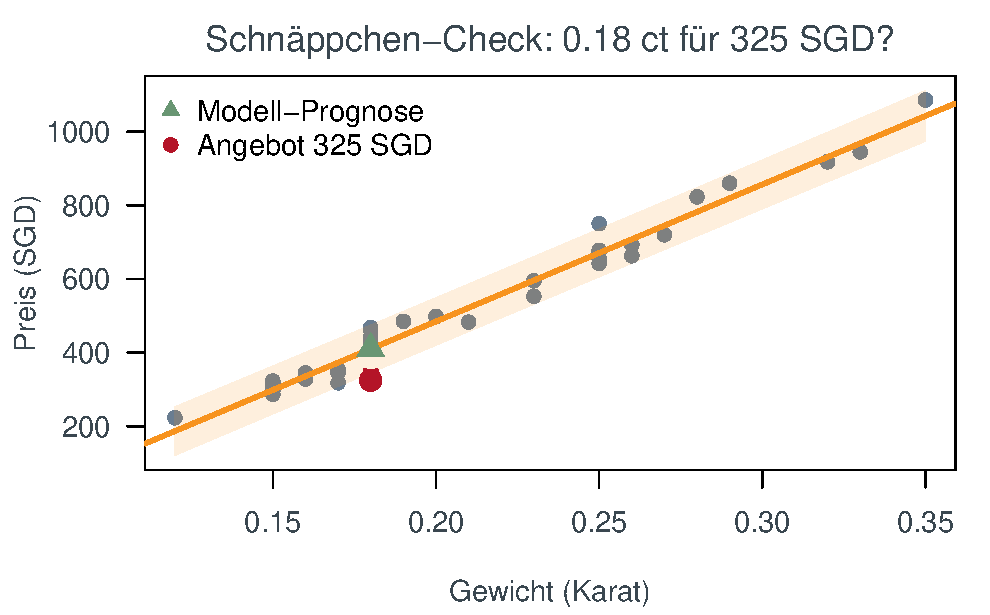
\includegraphics[width=\linewidth]{figures/dr_bargain.pdf}
\end{column}
\end{columns}
\end{frame}

\begin{frame}{Serie 5 --- Fazit}
\begin{itemize}
  \item \texttt{lm(price \textasciitilde{} weight)} liefert die
        kleinste-Quadrate-Gerade in einer Zeile
  \item \textbf{Steigung} = Mehrpreis pro Einheit; \textbf{Achsenabschnitt}
        oft nicht sinnvoll interpretierbar
  \item $R^2$ misst den erklärten Anteil, \textbf{RSE} den typischen Fehler
  \item das \textbf{Prognoseintervall} macht aus dem Modell eine
        konkrete Entscheidung (Schnäppchen ja/nein)
\end{itemize}
\vspace{0.3cm}
\begin{merke}[Übergang zu Serie 6]
Bisher: \textbf{ein} Prädiktor. Was, wenn wir \textbf{mehrere} haben ---
und diese sich gegenseitig ins Gehege kommen?
\end{merke}
\end{frame}

% ============================================================
\section{Serie 6 --- Multiple Regression}
% ============================================================

\begin{frame}{Die Aufgabe: Download-Zeiten}
\textbf{Datensatz \texttt{Download}} (80 Übertragungen): Übertragungszeit
(s), Dateigrösse (MB) und \emph{Stunden nach 8:00 Uhr}.

\vspace{0.3cm}
Wir erweitern das einfache Modell aus Serie 5:
\[
  \text{time} = b_0 + b_1\cdot\text{size}
  \quad\longrightarrow\quad
  \text{time} = b_0 + b_1\cdot\text{size} + b_2\cdot\text{hours}
\]

\begin{itemize}
  \item Was passiert mit der Steigung von \texttt{size}, wenn
        \texttt{hours} dazukommt?
  \item Lohnt sich der zweite Prädiktor überhaupt?
\end{itemize}

\begin{merke}[Leitfrage]
Zwei Prädiktoren, die fast \emph{dasselbe} messen --- Hilfe oder Problem?
\end{merke}
\end{frame}

\begin{frame}{Kernkonzept: marginale vs.\ partielle Steigung}
\begin{columns}[T]
\begin{column}{0.5\textwidth}
\textbf{Marginale Steigung}\\
(einfache Regression \texttt{time \textasciitilde{} size})
\begin{itemize}
  \item Effekt von \texttt{size} \alert{allein}
  \item ignoriert alle anderen Variablen
\end{itemize}
\vspace{0.3cm}
\textbf{Partielle Steigung}\\
(multiple Regression)
\begin{itemize}
  \item Effekt von \texttt{size}, \alert{wenn \texttt{hours} konstant
        gehalten wird}
  \item „bei sonst gleichen Bedingungen``
\end{itemize}
\end{column}
\begin{column}{0.48\textwidth}
\begin{merke}
Sind die Prädiktoren \textbf{unkorreliert}, sind marginale und partielle
Steigung praktisch gleich.

\vspace{0.2cm}
Sind sie \textbf{stark korreliert}, können sie sich dramatisch
unterscheiden.
\end{merke}
\end{column}
\end{columns}
\end{frame}

\begin{frame}[fragile]{Schritt 1: Die Prädiktoren ansehen}
\begin{columns}[T]
\begin{column}{0.5\textwidth}
\begin{rcode}
cor(download$size_mb,
    download$hours_after_8)
#>  0.988
\end{rcode}
\vspace{0.2cm}
Die Dateigrösse und „Stunden nach 8 Uhr`` sind mit $r = 0{,}99$ fast
\textbf{perfekt korreliert} --- sie tragen kaum eigene Information.

\vspace{0.2cm}
\alert{Frühwarnsignal} für Multikollinearität!
\end{column}
\begin{column}{0.48\textwidth}
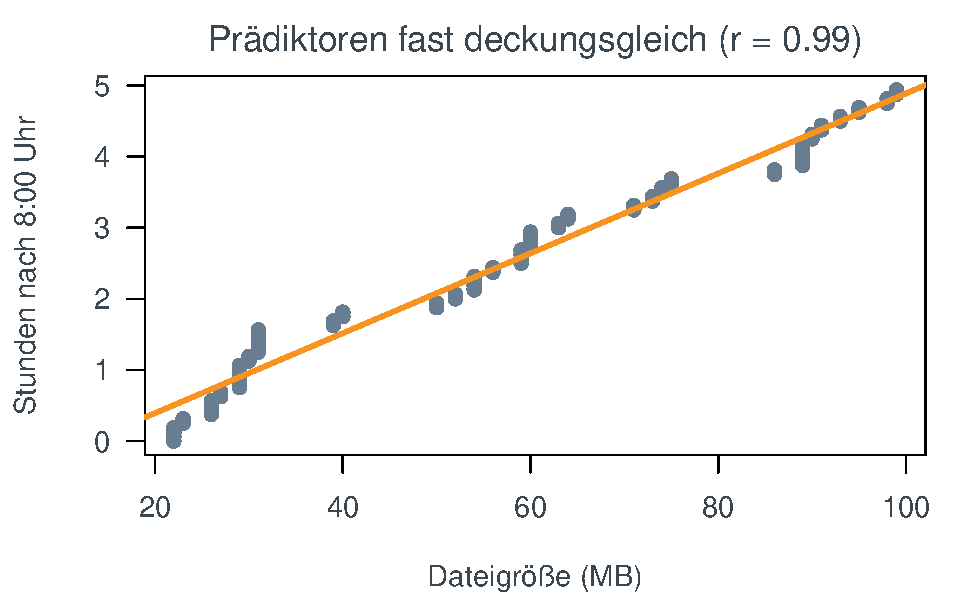
\includegraphics[width=\linewidth]{figures/dl_collinearity.pdf}
\end{column}
\end{columns}
\end{frame}

\begin{frame}[fragile]{Schritt 2--3: Beide Modelle schätzen}
\begin{rcode}
# marginal: nur size
lm(time_sec ~ size_mb, data = download)
# partiell: size + hours
lm(time_sec ~ size_mb + hours_after_8, data = download)
\end{rcode}
\vspace{0.2cm}
\centering
\renewcommand{\arraystretch}{1.25}
\begin{tabular}{lccc}
\toprule
Steigung \texttt{size} & Schätzung & Std.-Fehler & Bedeutung \\
\midrule
marginal (allein) & $0{,}313$ & $\mathbf{0{,}028}$ & präzise \\
partiell (mit \texttt{hours}) & $0{,}324$ & \alert{$\mathbf{0{,}180}$} & $6{,}4\times$ ungenauer \\
\bottomrule
\end{tabular}

\vspace{0.3cm}
Die Schätzung ändert sich kaum --- aber der \alert{Standardfehler
explodiert}.
\end{frame}

\begin{frame}{Kernkonzept: Multikollinearität}
\begin{columns}[T]
\begin{column}{0.42\textwidth}
\begin{center}
\begin{tikzpicture}[scale=0.95]
  \begin{scope}
    \clip (0.9,0) circle (1.5);
    \fill[LitmusAlert!40] (-0.9,0) circle (1.5);
  \end{scope}
  \draw[thick,LitmusPrimary] (-0.9,0) circle (1.5) node[left=1.1cm] {\small size};
  \draw[thick,LitmusAccent]  (0.9,0) circle (1.5) node[right=1.1cm] {\small hours};
  \node[font=\scriptsize,align=center] at (0,0) {fast\\alles\\gemeinsam};
\end{tikzpicture}
\end{center}
\end{column}
\begin{column}{0.56\textwidth}
Wenn zwei Prädiktoren fast dasselbe messen, kann das Modell ihre Effekte
\textbf{nicht sauber trennen}:
\begin{itemize}
  \item Schätzungen werden \alert{instabil} (riesige Standardfehler)
  \item Koeffizienten bekommen oft \alert{unsinnige Vorzeichen}
  \item Diagnose: \textbf{VIF} (Variance Inflation Factor)
\end{itemize}
\vspace{0.2cm}
Faustregel: $\text{VIF} > 10$ ist kritisch. Hier: \alert{VIF $= 42$}.
\end{column}
\end{columns}
\end{frame}

\begin{frame}[fragile]{Schritt 4: Diagnose --- bringt \texttt{hours} etwas?}
\begin{rcode}
summary(mod_multi)$coef        # Auszug
#>                Estimate Std. Error t value Pr(>|t|)
#> size_mb           0.324      0.180    1.80    0.076
#> hours_after_8    -0.186      3.162   -0.06    0.953
library(car); vif(mod_multi)
#>  size_mb  hours_after_8
#>     42.2           42.2
\end{rcode}
\vspace{0.2cm}
\begin{itemize}
  \item \texttt{hours}-Koeffizient \alert{negativ und völlig
        insignifikant} ($p = 0{,}95$) --- inhaltlich unsinnig
  \item $R^2$: $0{,}625$ (einfach) vs.\ $0{,}625$ (multipel) --- \alert{kein
        Gewinn}
  \item \textbf{Adjusted} $R^2$ \emph{sinkt} sogar ($0{,}620 \to 0{,}615$)
\end{itemize}
\end{frame}

\begin{frame}{Serie 6 --- Fazit}
\begin{itemize}
  \item Multiple Regression schätzt \textbf{partielle} Effekte: „bei sonst
        gleichen Bedingungen``
  \item Stark korrelierte Prädiktoren ($r = 0{,}99$) verursachen
        \alert{Multikollinearität}
  \item Symptome: explodierende Standardfehler, unsinnige Vorzeichen, VIF $\gg 10$
  \item Mehr Variablen $\ne$ besseres Modell --- \textbf{adjusted $R^2$} und
        F-Test entscheiden
\end{itemize}
\vspace{0.3cm}
\begin{merke}[Übergang zu Serie 7]
Der explodierende Standardfehler ist genau das Thema von Serie 7:
\textbf{Wie sicher sind unsere Koeffizienten überhaupt?}
\end{merke}
\end{frame}

% ============================================================
\section{Serie 7 --- Inferenz in der Regression}
% ============================================================

\begin{frame}{Die Aufgabe: Werbe-Budgets}
\textbf{Datensatz \texttt{Advertising}} (200 Märkte): Umsatz (\texttt{sales})
in Abhängigkeit von Werbe-Budgets für \texttt{TV}, \texttt{radio},
\texttt{newspaper}.

\vspace{0.3cm}
Wir fragen nicht mehr nur „\emph{wie gross} ist der Effekt?{}``, sondern:
\begin{enumerate}
  \item Wie \alert{präzise} ist die geschätzte TV-Steigung?
        (klassisches vs.\ Bootstrap-Konfidenzintervall)
  \item Welche Prädiktoren sind \alert{statistisch signifikant}?
        (t-Test, F-Test)
  \item Wie unterscheiden sich \alert{Konfidenz-} und
        \alert{Prognoseintervall}?
\end{enumerate}
\end{frame}

\begin{frame}{Kernkonzept: Von der Schätzung zur Unsicherheit}
Unsere Daten sind nur \textbf{eine Stichprobe}. Mit anderen 200 Märkten
bekämen wir leicht andere Koeffizienten.

\vspace{0.3cm}
\begin{columns}[T]
\begin{column}{0.5\textwidth}
\begin{konzept}[Konfidenzintervall]
Bereich, in dem der \textbf{wahre} Koeffizient mit 95\,\%
Wahrscheinlichkeit liegt.
\end{konzept}
\end{column}
\begin{column}{0.5\textwidth}
\begin{konzept}[Signifikanztest]
Ist der Effekt \textbf{unterscheidbar von Null}? Kleines $p \Rightarrow$
ja.
\end{konzept}
\end{column}
\end{columns}
\vspace{0.3cm}
\begin{merke}
Inferenz = von der Stichprobe auf die \textbf{Grundgesamtheit}
schliessen --- mit ehrlicher Angabe der Unsicherheit.
\end{merke}
\end{frame}

\begin{frame}[fragile]{Schritt 1--2: Modell und klassisches KI}
\begin{columns}[T]
\begin{column}{0.5\textwidth}
\begin{rcode}
mod_tv <- lm(sales ~ TV,
             data = Advertising)
confint(mod_tv)
\end{rcode}
\begin{rout}
              2.5 %  97.5 %
(Intercept)  6.1297  7.9355
TV           0.0422  0.0528
\end{rout}
\vspace{0.2cm}
\small $\hat b_1 = 0{,}0475$: pro zusätzlichem \$1000 TV-Budget rund
\textbf{47{,}5} mehr verkaufte Einheiten. Hoch signifikant
($p \approx 10^{-42}$).
\end{column}
\begin{column}{0.48\textwidth}
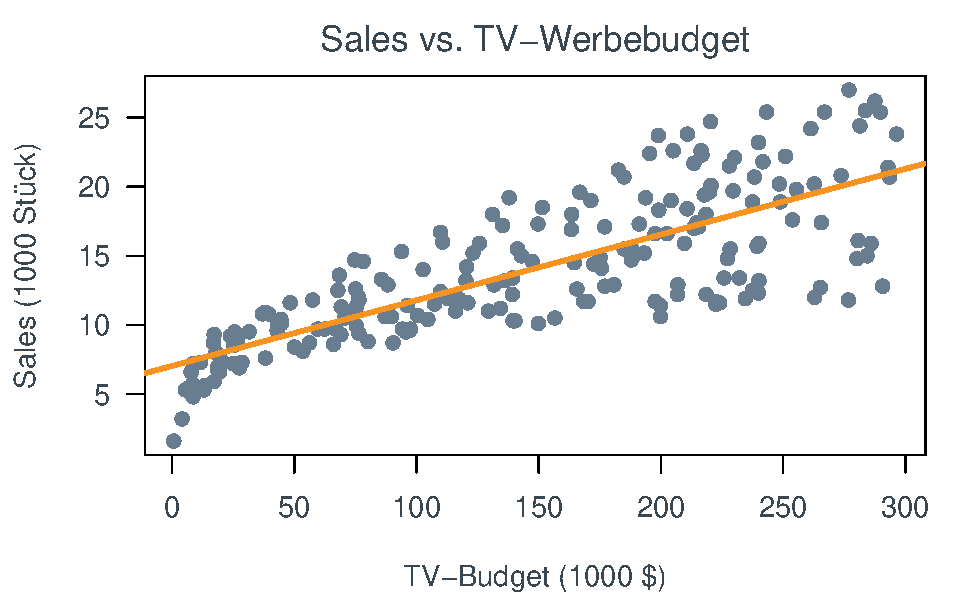
\includegraphics[width=\linewidth]{figures/adv_scatter.pdf}
\end{column}
\end{columns}
\vspace{0.1cm}
\centering\small
95\,\%-KI für TV: $[0{,}0422,\ 0{,}0528]$ --- klar oberhalb von 0.
\end{frame}

\begin{frame}{Kernkonzept: Der Bootstrap}
\textbf{Idee:} Statt eine Formel zu glauben, simulieren wir die
Unsicherheit aus den Daten selbst.

\vspace{0.2cm}
\begin{center}
\begin{tikzpicture}[>=Stealth, font=\small,
   box/.style={draw, rounded corners, minimum width=2.7cm, minimum height=1.1cm,
               text width=2.5cm, align=center}]
  \node[box, fill=LitmusPrimary!10]   (d) at (0,0)   {Daten\\($n=200$)};
  \node[box, fill=LitmusSecondary!25] (s) at (4.4,0) {Stichprobe\\\emph{mit Zurücklegen}};
  \node[box, fill=LitmusAccent!12]    (m) at (8.8,0) {$\hat b_1$ schätzen};
  \draw[->,thick] (d)--(s) node[midway,above,font=\scriptsize]{ziehen};
  \draw[->,thick] (s)--(m) node[midway,above,font=\scriptsize]{\texttt{lm()}};
  \draw[->,thick,LitmusIncorrect] (m.south) -- ++(0,-0.7) -| (d.south)
    node[midway,below=2pt,font=\scriptsize,LitmusIncorrect]{5000$\times$ wiederholen};
\end{tikzpicture}
\end{center}
\vspace{0.2cm}
Die \alert{Streuung der 5000 Schätzungen} ist direkt das
Konfidenzintervall --- ganz ohne Verteilungsannahme.
\end{frame}

\begin{frame}[fragile]{Schritt 3: Bootstrap-KI und Vergleich}
\begin{columns}[T]
\begin{column}{0.5\textwidth}
\begin{rcode}
library(mosaic)
set.seed(123)
simcoef <- do(5000) *
  coef(lm(sales ~ TV,
      data = resample(Advertising)))
quantile(simcoef$TV,
         c(0.025, 0.975))
#>   0.0419   0.0531
\end{rcode}
\end{column}
\begin{column}{0.48\textwidth}
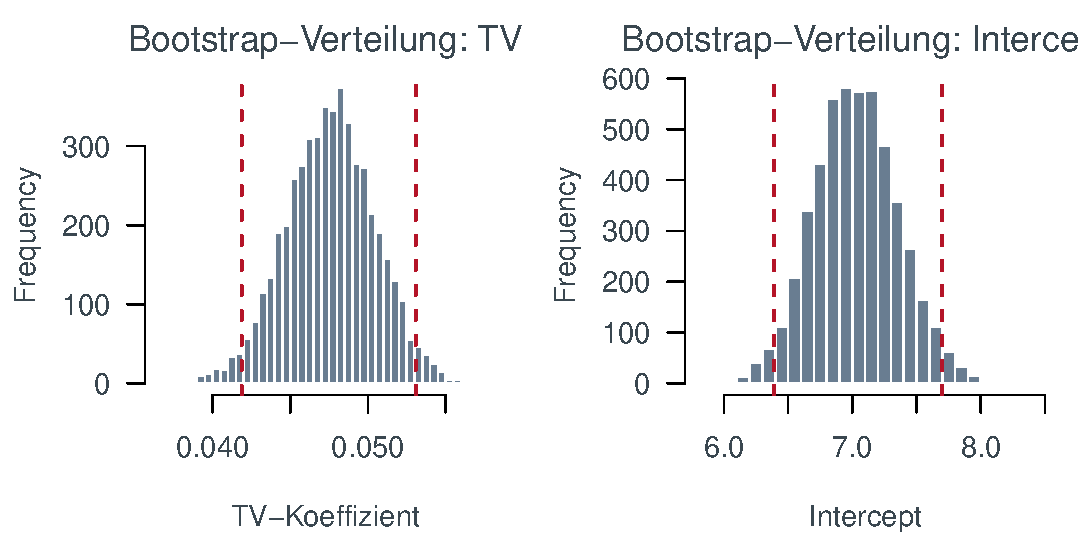
\includegraphics[width=\linewidth]{figures/adv_boot.pdf}
\end{column}
\end{columns}
\vspace{0.15cm}
\centering
\begin{tabular}{lcc}
\toprule
95\,\%-KI für TV & untere & obere \\
\midrule
klassisch (\texttt{confint}) & $0{,}0422$ & $0{,}0528$ \\
Bootstrap (5000) & $0{,}0419$ & $0{,}0531$ \\
\bottomrule
\end{tabular}

\vspace{0.15cm}
\small Praktisch identisch --- die klassischen Annahmen passen hier gut.
\end{frame}

\begin{frame}[fragile]{Schritt 4: Multiple Regression --- alle Kanäle}
\begin{rcode}
mod_full <- lm(sales ~ TV + radio + newspaper, data = Advertising)
summary(mod_full)$coef
\end{rcode}
\begin{rout}
            Estimate Std. Error t value Pr(>|t|)
(Intercept)  2.93889    0.31191   9.422  < 2e-16 ***
TV           0.04576    0.00139  32.809  < 2e-16 ***
radio        0.18853    0.00861  21.893  < 2e-16 ***
newspaper   -0.00104    0.00587  -0.177    0.860
\end{rout}
\vspace{0.15cm}
\texttt{TV} und \texttt{radio} hoch signifikant ---
\texttt{newspaper} mit $p = 0{,}86$ \alert{nicht von Null
unterscheidbar}.
\end{frame}

\begin{frame}{Kernkonzept: t-Test vs.\ F-Test}
\begin{columns}[T]
\begin{column}{0.5\textwidth}
\begin{konzept}[t-Test]
Prüft \textbf{einen einzelnen} Koeffizienten:\\
$H_0: \beta_j = 0$.\\[2pt]
Steht in jeder Zeile der \texttt{summary}-Ausgabe (Spalte
\texttt{Pr(>|t|)}).
\end{konzept}
\end{column}
\begin{column}{0.5\textwidth}
\begin{konzept}[F-Test]
Prüft \textbf{mehrere} Koeffizienten gemeinsam, bzw.\ vergleicht zwei
\textbf{geschachtelte} Modelle:\\
„Bringt die Zusatzvariable als Gruppe etwas?{}``
\end{konzept}
\end{column}
\end{columns}
\vspace{0.3cm}
\begin{merke}
Für „lohnt sich \texttt{newspaper}?{}`` vergleichen wir das Modell
\emph{mit} und \emph{ohne} \texttt{newspaper} per F-Test (\texttt{anova}).
\end{merke}
\end{frame}

\begin{frame}[fragile]{Schritt 5: Modellvergleich per F-Test}
\begin{rcode}
mod_red  <- lm(sales ~ TV + radio, data = Advertising)
anova(mod_red, mod_full)
\end{rcode}
\begin{rout}
  Res.Df    RSS Df Sum of Sq      F Pr(>F)
1    197 556.91
2    196 556.83  1   0.08872 0.0312  0.860
\end{rout}
\vspace{0.2cm}
\begin{itemize}
  \item $F = 0{,}03$, $p = 0{,}86$ $\Rightarrow$ \texttt{newspaper} liefert
        \alert{keinen} signifikanten Zusatzbeitrag
  \item Der $p$-Wert stimmt mit dem t-Test überein (bei \emph{einer}
        Variable identisch)
  \item \textbf{Entscheidung:} \texttt{newspaper} entfernen --- einfacheres
        Modell bevorzugen
\end{itemize}
\end{frame}

\begin{frame}{Kernkonzept: Konfidenz- vs.\ Prognoseintervall}
Beide drehen sich um die Frage „Wie viel \texttt{sales} bei TV=200,
radio=30?{}`` --- aber sie beantworten \textbf{verschiedene} Fragen:

\vspace{0.2cm}
\begin{columns}[T]
\begin{column}{0.5\textwidth}
\begin{konzept}[Konfidenzintervall (CI)]
Wo liegt der \textbf{Mittelwert} der Sales über \emph{viele} Märkte mit
diesen Budgets? \\ $\rightarrow$ \textbf{eng}
\end{konzept}
\end{column}
\begin{column}{0.5\textwidth}
\begin{konzept}[Prognoseintervall (PI)]
Wo liegt \textbf{ein einzelner, neuer} Markt? \\
$\rightarrow$ \textbf{breiter} (zusätzliche Einzel-Streuung)
\end{konzept}
\end{column}
\end{columns}
\vspace{0.3cm}
\centering
Das PI enthält das CI \emph{immer} --- es trägt eine zusätzliche
Unsicherheitsquelle.
\end{frame}

\begin{frame}[fragile]{Schritt 6: CI und PI berechnen}
\begin{columns}[T]
\begin{column}{0.52\textwidth}
\begin{rcode}
nv <- data.frame(TV = 200, radio = 30)
predict(mod_red, nv,
        interval = "confidence")
#>    fit    lwr    upr
#> 17.71  17.42  18.01
predict(mod_red, nv,
        interval = "prediction")
#>    fit    lwr    upr
#> 17.71  14.38  21.04
\end{rcode}
\small CI-Breite $\approx 0{,}6$, PI-Breite $\approx 6{,}7$ ---
\textbf{gut 10$\times$ breiter}.
\end{column}
\begin{column}{0.46\textwidth}
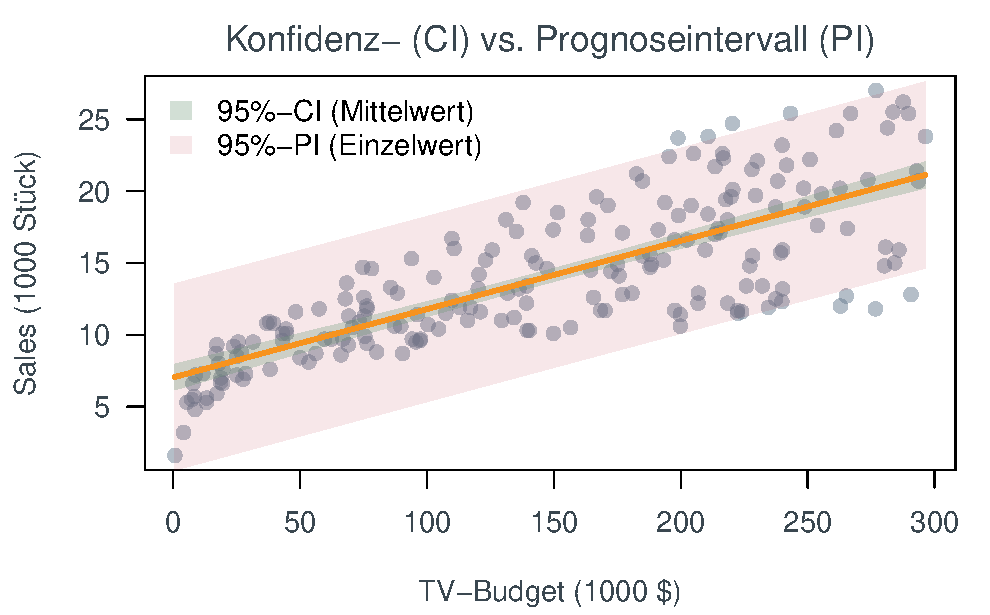
\includegraphics[width=\linewidth]{figures/adv_cipi.pdf}
\end{column}
\end{columns}
\end{frame}

% ============================================================
\section{Zusammenfassung}
% ============================================================

\begin{frame}{Die drei grossen Ideen}
\begin{columns}[T]
\begin{column}{0.32\textwidth}
\begin{konzept}[Serie 5]
\textbf{Anpassen \& nutzen}\\[3pt]
Kleinste Quadrate, $b_0/b_1$, $R^2$/RSE --- und das
\textbf{Prognoseintervall} für echte Entscheidungen.
\end{konzept}
\end{column}
\begin{column}{0.32\textwidth}
\begin{konzept}[Serie 6]
\textbf{Mehrere Prädiktoren}\\[3pt]
\textbf{partielle} Steigung „bei sonst Gleichem`` --- und die Gefahr der
\textbf{Multikollinearität}.
\end{konzept}
\end{column}
\begin{column}{0.32\textwidth}
\begin{konzept}[Serie 7]
\textbf{Unsicherheit}\\[3pt]
KI (klassisch \& \textbf{Bootstrap}), t-/F-Test, CI vs.\ PI ---
\textbf{wie sicher} sind wir?
\end{konzept}
\end{column}
\end{columns}
\vspace{0.5cm}
\begin{merke}[Roter Faden]
Ein Modell ist erst vollständig, wenn wir nicht nur die \textbf{Punkt}schätzung
kennen, sondern auch ihre \textbf{Unsicherheit} ehrlich beziffern.
\end{merke}
\end{frame}

\begin{frame}[standout]
Fragen?
\end{frame}

\end{document}
